% outline discussion
% 1. Symbolic restructuring
% 2. DQN results 
% 3. Problems with StarCraft
% 4. Can we make the interface better? 

\chapter{Discussion}

\section{Project Completion}

Despite the short amount of time that we had at disposition to complete the
project, we believe we have successfully implemented all the initial specifications:

\begin{itemize}
\item We built a robust interface to StarCraft.
\item We managed to connect such interface to a state-of-the-art tensor library.
\item We implemented a couple of baseline reinforcement learning algorithms to
  work with simple StarCraft domains.
\end{itemize}

All of this was done with limited experience in network programming and no prior
knowledge of BWAPI, Windows API programming or Torch. The downside is that the
development of the entire pipeline took a much greater amount of time than
expected (and well over twice the assigned 400 hours), most of which ended up
being spent in the implementation of the various internal interfaces between the
different modules and environments.

Moreover while the initial idea was to create modules to cluster the useful
parts of the game state in such a way that researchers would only have to
interact with the client code when ``configuring'' the reward function
\footnote{If needed. In reality this can already be done in most cases on the
  agent side with the aid of the game state data.}, some of the initials design
decisions made the implementation significantly harder to modify and debug. This
became especially evident when we realised towards the end of the project that
to add the necessary degree of control over the game settings we would have had
to change the structure of BWLE's modules to allow the server to interact not
only with BWAPI but also with the actual StarCraft process.

\section{Challenges for machine learning approaches}

Now that the framework is in a usable state, it's time to think about tackling
some of the fundamental problems in reinforcement learning and general
artificial intelligence.

\subsection{State exploration as a policy}
As previously mentioned, with most of the roms used within ALE the visual data
contains the full state of the game. That is, assuming we have a good
understanding of the score function, the image given by ALE essentially gives us
all the information we need to model the most useful action at any given time
with reasonable results. In Starcraft the visual feedback purely represents the
state of the game at a specific point in the map - point usually chosen by the
player through keyboard or mouse actions - and unless the user puts time and
effort in dynamically exploring the map to update his world knowledge, they
can't get an idea of the general state of the game a part from looking at the
extremely compressed minimap (Figure \ref{fig:one_star}).

\begin{figure}[h]
    \centering
    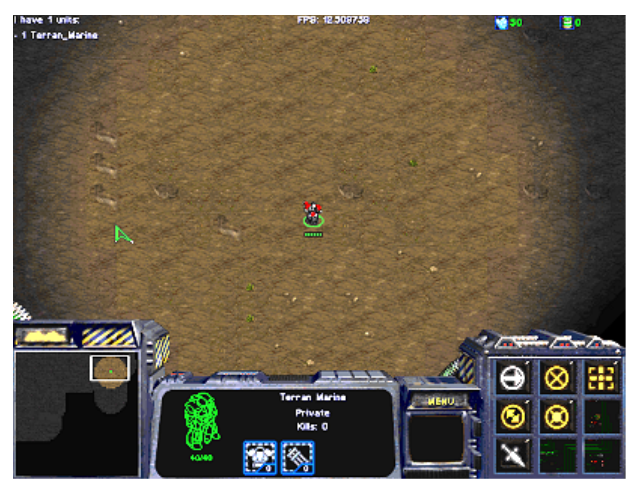
\includegraphics[width=0.5\textwidth]{ch6/star_one}
    \caption{Standard StarCraft game screen that the player needs to interact
      with. The minimap is on the bottom-left; black areas are not yet
      discovered (and therefore not observable), grey areas have been discovered
      but are not fully observable anymore (topology of the map is known, unit
      or resources status is not) and light brown areas are observed areas with
      full observability in terms of game state (symbolical). The white
      rectangle signals the visible area at the current window position.}
    \label{fig:one_star}
\end{figure}

Additionally the minimap is also affected by the so-called Fog of War, a feature
in most RTS games that prevents players from observing the state of locally
explored but unobserved zones at a specific time. This means that to fully win
the game the player is forced to continuously explore the state of the game,
regardless of whether they have a more or less complete notion of the topology
of the map. In reality, Starcraft allows us to cheat and disable the Fog of War,
making exploration a one-shot process i.e. once the map is explored it’ll be
“observable” through the entirety of the match.

\begin{figure}[h]
    \centering
    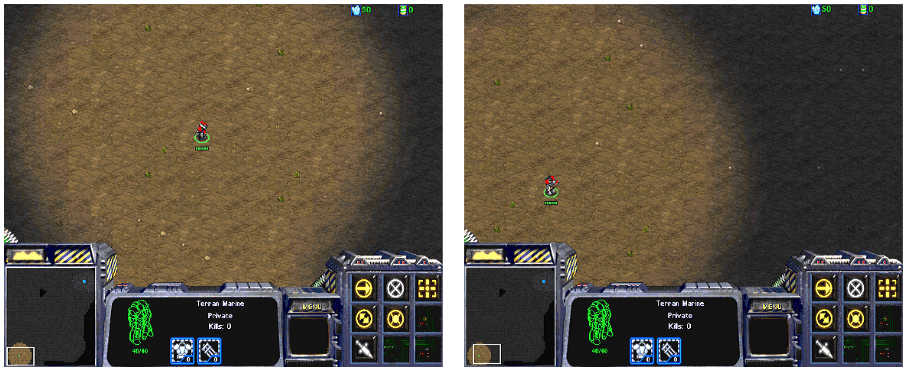
\includegraphics[width=\textwidth]{ch6/double_star}
    \caption{The variance in visual input between the two windows is as seen
      very high, because not only the relative position of the unit changes, but
      the entirety of the space changes significantly.}
    \label{fig:double_star}
\end{figure}

Starcraft’s visual feedback by itself (i.e. even without encoded features) is
therefore essentially non-Markovian in how it represents the state of the game.
Starcraft players are required to move the window to gain information, and the
image changes drastically depends on where the window is (Figure
\ref{fig:double_star}), so unless there is some form of memory to collect the
game state, we cannot only use the visual data as input. Our conjecture is that
creating an encoded representation of the entire state of game is by itself an
unsolved mixed deep learning (representation) and RL problem, as the variance in
the input is simply too large and it's entirely based on the learnt policy for
both unit actions and screen/environment actions.

\subsection{Hierarchical Decision-Making}

In Chapter 2 we have discussed some work in Hierarchical Reinforcement Learning
that could be used in principle to tackle StarCraft, however no particular model
seems to fit all the requirements of the platform, especially if we take and
end-to-end approach to the problem. It's probably fair to speculate that
similarly to AlphaGo, a reinforcement learning framework will need some amount
of strong supervision to learn good overall strategies and hand-tuned feature
extractors.

% Cover Russell work
% Cover Policy reuse
% include also policy distillation?
% Cover counterfactual reasoning

\subsection{Data-Efficient Machine Learning}

Reinforcement learning and deep learning algorithms are alike in the
fact that they require many data samples to correctly estimate underlining
models, in fact those systems have now become hugely popular as scalable
solutions for tackling problems related to object recognition, image
segmentation and speech processing, all of which have relevant data available in
great quantities.

If we look at most StarCraft games we can notice instead that while some
strategies are predominant in certain parts of match (e.g. build workers and
scouts to explore the map and gather resources during the early stages of the
game), a lot of strong tactical moves are extremely rare and will appear only
under precise conditions. This is why we must develop interactive mechanisms to
use those powerful techniques in a one-shot fashion. The machine learning and
robotics communities has started tackling this problem
\citep{deisenroth2015gaussian, assael2015data, kingma2014semi,
  rasmus2014denoising}, but no clear solution has emerged so far. StarCraft
together with our framework should provide the perfect environment to explore
those scenarios.

\subsection{Text-Based Expert Knowledge Distillation}

\section{Future Work}

Before releasing the platform there are a few things we need to carry out to
make the user experience more straightforward.

\subsection{Design Clean-up}

Now that we know the quirks of both BWAPI and StarCraft itself, we can adjust
the design of the client manager modules to better match BWAPI's internal
structure. Here's some ways we could achieve this:

\begin{itemize}
\item The client could be split in three different asynchronous modules: a
  StarCraft handler to control Windows and the StarCraft process, a Game State
  collector to observe and collect the state using BWAPI and WinAPI, and a
  networking interface to deal with the external interface.
\item \texttt{BWAPIClient} could be expanded to add the ability to fully control
  the game in a similar fashion, simplifying our overall architecture. This way
  we could easily write a background daemon process to produce BWLE virtual
  machines with underlying BWLE processes running all the time, facilitating
  multi-client experiments.
\end{itemize}

Additionally we would like to replace the protobuf serialisation system with
some slightly more used systems such as \texttt{Json} or \texttt{XML}. This
would be helpful to integrate the architecture with web systems and would also
allow a more easily accessible (and human readable) data representation by
potentially only losing some speed when parsing the structure.

\subsection{Full Linux compatibility}

The great majority of AI and machine learning researchers do not use Windows as
their development environment. Having to use a VM to host the StarCraft client
and the interface means that there is a higher cost then normal associated with
using the platform (that is, providing a simple installation script or a working
out-the-box environment is not an immediate process).

In the past some parts of BWAPI were made to be compatible with other compilers
and WINE, a Linux environment that tries to reproduce the Windows API and
provide tools for running Windows software on unix platforms. Porting the
entirety of our pipeline over Linux would mean being able to significantly
simplify the integration with other state-of-the-art machine learning systems
and remove some of the difficulties in using the platform (as the installation
can be cumbersome). 


\subsection{ROS integration}

ROS is an open-source framework designed to aid the development of robotic
software. It is essentially an extremely useful collection of build tools,
programming languages interfaces, simulation and visualisation software and
packages that allow the robotics community worldwide to share research with a
unified interface.

A wide variety of robotics communities regularly release packages for ROS, and
while most of them are not directly applicable to the StarCraft domains, it
would be extremely beneficial to link the platform to research groups work on
hierarchical planning and reasoning. As ROS is available on both Linux, Windows
and OSX, it would also allow us to define a unified and distributed networking
interface based on the publisher-subscriber messaging pattern and greatly
simplify the creation of a StarCraft-based simulation environment.


\section{Chapter Summary}

We have discovered that StarCraft is challenging for a large variety of reasons,
most of which are problems effectively shared with a lot of other RTS games.
Regardless, we don't believe we would have managed to reach the same results
using any of the other available RTS platforms had we not had something
equivalent to BWAPI.
 